% Shared manuscript semantics. The document class and publication-specific
% presentation are selected by dashvmc-preprint.tex or dashvmc-submission.tex.
\ifdashvmcsubmission
  \usepackage[utf8]{inputenc}
  \usepackage[T1]{fontenc}
\fi
\usepackage{hyperref}
\usepackage{url}
\usepackage{booktabs}
\usepackage{amsfonts}
\usepackage{amsmath}
\usepackage{microtype}
\usepackage{xcolor}
\usepackage{graphicx}
\usepackage{placeins}

\ifdashvmcsubmission
  \definecolor{citeblue}{HTML}{4A90E2}
  \hypersetup{
    colorlinks=true,
    citecolor=citeblue,
    linkcolor=citeblue,
    urlcolor=citeblue,
    pdftitle={DashVMC: Real-Time Discrete World Model Control in Geometry Dash},
    pdfauthor={}
  }
\else
  \hypersetup{
    pdftitle={DashVMC: Real-Time Discrete World Model Control in Geometry Dash},
    pdfauthor={Florent Tariolle}
  }
\fi

% Architectural constants.
\newcommand{\hdim}{384}
\newcommand{\nheads}{8}
\newcommand{\nlayers}{8}
\newcommand{\nctx}{4}
\newcommand{\ntokens}{64}
\newcommand{\vocabsize}{1000}
\newcommand{\fsqlevels}{[8,5,5,5]}
\newcommand{\gridsize}{8 \times 8}
\newcommand{\imgsize}{64 \times 64}
\newcommand{\ctrlparams}{45{,}546}

\newcommand{\dashvmcabstract}{%
World-model agents are usually evaluated in simulators that can wait for the policy; live games impose the opposite constraint, requiring capture, prediction, and action before the next frame.
We present \emph{DashVMC}, a discrete world-model agent that plays Geometry Dash from screen pixels.
A Finite Scalar Quantization (FSQ) tokenizer compresses Sobel-filtered observations into discrete token grids, a block-causal transformer predicts action-conditioned transitions, and a lightweight actor--critic is initialized by behavioural cloning (BC) and subsequently optimized with Proximal Policy Optimization (PPO) in latent rollouts.
Training uses approximately 2 hours of gameplay captured at a nominal 30-FPS cadence, including less than 20 minutes of expert segments; all learning is offline, without any real-environment interaction by the agent.
Across three independent controller seeds, PPO has higher mean live survival than its exact retained parent BC on every official level for every seed, with the largest gains on the first two levels.
Deployed locally, the complete capture-to-action pipeline supports reactive control at 60 FPS on a consumer GPU.
Beyond control, the learned dynamics generate interactive, open-ended visual level continuations that can remain plausible over extended rollouts.
These results demonstrate that a specialized world model can jointly support imagined policy optimization, interactive generation, and real-time deployment.%
}

\ifdashvmcsubmission
  \title{DashVMC: Real-Time Discrete World Model Control\\in Geometry Dash}
  \author{Anonymous Author(s)}
\else
  \title{%
    DashVMC\\[0.1em]
    {\large\color{black!70}Real-Time Discrete World Model Control in Geometry Dash}%
  }
  \author{Florent Tariolle}
  \affiliation{INSA Rouen Normandy}
  \abstract{\dashvmcabstract}
  \metadata[Project page]{\href{https://tariolle.github.io/dash-vmc/}{tariolle.github.io/dash-vmc}}
  \metadata[Code]{\href{https://github.com/Tariolle/dash-vmc}{github.com/Tariolle/dash-vmc}}
  \correspondence{\email{florent.tariolle@insa-rouen.fr}}
\fi

\begin{document}

\maketitle

\ifdashvmcsubmission
  \begin{abstract}
    \dashvmcabstract
  \end{abstract}
\fi

\section{Introduction}
\label{sec:intro}

A world model learns an environment's transition dynamics, conventionally written \(p_\theta(s_{t+1}\mid s_t,a_t)\): given a state \(s_t\) and action \(a_t\), it predicts the state that follows~\citep{lecun2022path}.
When privileged environment state is unavailable, as here, the model instead operates on a learned latent representation inferred from recent observations and actions.
Rolling the model forward allows an agent to improve its policy in imagination rather than through additional interaction with the real environment~\citep{ha2018world}.
Discrete approaches such as IRIS encode images into tokens and model their evolution with an autoregressive transformer~\citep{micheli2023iris}, whereas DIAMOND uses diffusion to preserve fine visual detail~\citep{alonso2024diamond}.
DashVMC instead targets a joint systems requirement: inexpensive imagined transitions for policy optimization together with a decoder-free live path that reuses the dynamics model's temporal state.
It follows IRIS's discrete autoregressive formulation across frames, but predicts each next token grid in parallel and is adapted to an approximately two-hour offline corpus and a live-control setting.

Regardless of model class, most world-model agents are evaluated in synchronous, step-based environments whose simulation advances only when the agent submits an action.
Controlling a live, non-paused application imposes an additional wall-clock constraint: screen capture, preprocessing, state estimation, policy inference, and action dispatch must finish before the action becomes stale.

Geometry Dash is a small but unforgiving test of this contract.
The avatar moves continuously, the action space is binary, and a mistimed jump causes immediate death.
Levels are deterministic, but the agent observes only captured pixels and acts through keyboard events; it does not receive emulator state during control.
This combination makes Geometry Dash a practical deployment stress test: can a pixel-based world-model agent close the live capture-to-action loop quickly and precisely enough for narrow timing windows on a consumer GPU?

DashVMC adopts the broad perception--dynamics--control organization introduced by World Models~\citep{ha2018world}.
An FSQ tokenizer~\citep{mentzer2024fsq} encodes Sobel edge maps.
An action-conditioned transformer world model predicts the next token grid from the recent latent context and a chosen action, enabling autoregressive imagined rollouts of the controller's decisions.
The controller receives both the current observation grid and the transformer's temporal state; after a short BC warm start, it is optimized by PPO~\citep{schulman2017ppo} entirely in rollouts generated by the frozen world model.
At deployment, neither decoding nor next-frame prediction is executed: the encoder, transformer context pass, and controller run once per frame, while policy optimization has already happened offline.

This is a systems co-design contribution rather than a new generic world-model primitive.
The 64-token visual grid bounds live perception and context-encoding cost, while the parallel next-frame predictor bounds the cost of imagined rollouts; explicit action conditioning permits counterfactual rollouts; BC avoids an expensive random-policy transient; and GPU-resident state plus captured execution remove avoidable synchronization from the live path.
Our contributions are:
\begin{enumerate}
  \item an end-to-end discrete world-model agent for pixel-based control of the original, non-paused Geometry Dash game, whose parallel imagined transition fits within a 30-FPS frame period and whose decoder-free capture-to-action path sustains a 60-FPS live cadence on a consumer GPU; and
  \item an offline training pipeline using approximately two hours of captured gameplay, including less than 20 minutes of expert segments, that initializes a lightweight controller with BC and optimizes it with PPO entirely in autoregressive rollouts of the frozen action-conditioned world model, without any real-environment interaction by the agent during learning.
\end{enumerate}
We evaluate these contributions through three retained BC-to-PPO controller pairs on three official and two auxiliary layouts, matched-action interventions, end-to-end latency profiling, and qualitative open-ended rollouts and failure analysis.

\section{Related work}
\label{sec:related}

\paragraph{World models and imagination.}
The original Vision--Memory--Controller pipeline compressed observations with a VAE, modeled latent dynamics with an MDN--RNN, and demonstrated in VizDoom that a compact controller could be optimized entirely in learned dreams and transferred to the real environment~\citep{ha2018world}.
Subsequent imagination-based agents explore different representations and dynamics models: IRIS, the closest architectural reference for DashVMC, combines a discrete autoencoder with an autoregressive transformer for data-efficient Atari learning~\citep{micheli2023iris}; \(\Delta\)-IRIS separates stochastic changes into discrete tokens from continuous context tokens to reduce sequence cost~\citep{micheli2024deltairis}; and DIAMOND uses diffusion without discrete compression for imagination-trained control and also demonstrates an interactive Counter-Strike neural game engine~\citep{alonso2024diamond}.
DreamerV3 demonstrates broad control with categorical recurrent state-space latents~\citep{hafner2025dreamerv3}, while TWISTER augments transformer world-model training with action-conditioned contrastive predictive coding to learn temporal representations over longer horizons~\citep{burchi2025twister}.
At larger generative scales, related action-conditioned simulators include MIRA, which models tightly coupled four-player Rocket League dynamics with latent diffusion~\citep{hu2026mira}; MineWorld, which autoregressively models interleaved discrete visual and action tokens with parallel spatial decoding~\citep{guo2025mineworld}; and Matrix-Game 2.0, which uses few-step diffusion for streaming generation~\citep{he2025matrixgame}.
Within Geometry Dash specifically, earlier screenshot-based control used direct DQN and imitation learning under a DLL-fabricated timestep, and highlighted that narrow jump windows can make nearly identical frames require different actions~\citep{li2017geometrydash}.
Our protocol leaves the game clock running and supplies the controller with temporal context through the learned world model.

\paragraph{FSQ tokenization and policy initialization.}
FSQ replaces learned vector-quantization codebooks with bounded scalar levels, avoiding commitment losses and codebook collapse while exposing an integer coordinate lattice~\citep{mentzer2024fsq}; we use the improved iFSQ bounding function~\citep{lin2026ifsq}.
For policy initialization, demonstration-based RL has repeatedly shown that supervised behaviour can reduce the expensive early interaction phase~\citep{hester2018deep,baker2022vpt}.
Here demonstrations only initialize the controller: the final policy is selected after PPO improvement in the learned environment.

\paragraph{Representation anchors and alternatives.}
Joint-embedding prediction can avoid spending capacity on high-magnitude input detail that is irrelevant or unpredictable from context~\citep{vanassel2025joint}, and LeWorldModel demonstrates stable end-to-end predictive learning from pixels with continuous latents~\citep{maes2026leworldmodel}.
DashVMC instead applies deterministic preprocessing that converts each cropped RGB capture to grayscale and then to a Sobel edge map, removing much appearance detail before learning and making reconstruction a comparatively inexpensive anchor for the shared discrete token space.
Among discrete tokenizers, Gaussian Quant reports stronger rate--distortion performance than FSQ on large image benchmarks~\citep{xu2025gq}.
Whether those gains transfer to low-resolution Sobel edge maps and downstream world-model control remains untested.

\section{DashVMC}
\label{sec:method}

The three modules are trained sequentially: \(V\) and \(M\) are frozen before controller fitting, and the selected controller is frozen for deployment.
Figure~\ref{fig:pipeline} separates the imagined PPO path from the live reactive path.

\begin{figure}[ht!]
  \centering
  
\includegraphics[width=\textwidth]{figures/pipeline.pdf}
  \caption{DashVMC policy improvement and deployment. \textbf{(a)} PPO rollouts start from a recorded \(K=4\) token--action context. The frozen world model predicts \(\hat{\mathbf z}_{\mathrm{next}}\) and \(p_{\mathrm{death}}\) while returning context feature \(\mathbf h\); the controller acts from the first imagined step, and the predicted grid and selected action are appended to the rolling context. The first four transitions form a controller-active grace period: they replace the recorded seed and are excluded from PPO to filter deaths likely already unavoidable from the initial context. PPO updates only \(C\). \textbf{(b)} During live control, all weights are frozen. \(V\) encodes captured frames and \(M\) performs context prefill only to produce \(\mathbf h_t\). The controller receives the current grid \(\mathbf z_t\) directly together with \(\mathbf h_t\) and dispatches the keyboard action; neither next-grid prediction nor decoding is run.}
  \label{fig:pipeline}
\end{figure}

\subsection{Visual tokenization}
\label{sec:fsq}

Each RGB capture is cropped, converted to grayscale, filtered with Sobel edges, and resized to \(\imgsize\).
A convolutional autoencoder maps the result through three stride-2 stages to a four-channel \(\gridsize\) latent map.
Each spatial vector is independently quantized with iFSQ levels \(\fsqlevels\), using the bounding function \(2\operatorname{sigmoid}(1.6z)-1\), and yields \(\ntokens\) token IDs from \(\vocabsize\) implicit codes.
The tokenizer is trained on adjacent frame pairs with pixel-MSE reconstruction plus temporal slowness and latent-uniformity regularizers~\citep{xia2025grwm}.
The encoder and decoder contain \(941{,}924\) and \(941{,}921\) trainable parameters, respectively.
After selection, the encoder is frozen and the decoder is retained only for visualizing dreams.

\subsection{Action-conditioned dynamics}
\label{sec:transformer}

The dynamics model has \(\nlayers\) transformer layers, width \(\hdim\), and \(\nheads\) attention heads, for \(14{,}723{,}520\) unique trainable parameters including \(141{,}120\) in the contrastive predictive coding (CPC) training heads.
Each frame block contains 64 visual tokens and one \textsc{alive}/\textsc{death} status token; action tokens are inserted between blocks.
Given \(K=\nctx\) observed frame--action pairs, a final masked block requests the next frame.
The resulting sequence has \(K(65+1)+65=329\) positions; every target-frame position receives a learned \texttt{[MASK]} embedding, so no target token is exposed during training.
Attention is bidirectional within a frame and causal across frame/action blocks, so all next-frame positions are predicted in one forward pass without seeing their targets.
Factored 3D rotary embeddings encode row, column, and time, with spatial and temporal bases 10 and 10,000; status and action tokens use the grid centre coordinates~\citep{su2024rope}.
The status logits supply the rollout termination score, and the final context state \(\mathbf h_t\in\mathbb R^{\hdim}\) summarizes recent dynamics for the controller.
In the reported interleaved sequence, this state is taken from the most recent action-token position.
Death frames are oversampled \(5\times\) during training to prevent the overwhelmingly common \textsc{alive} class from admitting a trivial always-alive solution.
Consequently, the \textsc{death} score from a two-class softmax over \textsc{alive}/\textsc{death} is used operationally rather than interpreted as a calibrated environment probability.

We add TWISTER's action-conditional contrastive predictive-coding loss with weight 0.1~\citep{burchi2025twister}: for each future offset \(k\leq K\), an MLP predicts \(\mathbf h_{t+k}\) from \(\mathbf h_t\) and the intervening actions and is scored with in-batch InfoNCE~\citep{oord2018cpc}.
We also independently replace 5\% of context tokens uniformly and 5\% with adjacent FSQ codes.
The token loss uses focal modulation~\citep{lin2017focal} and structured label smoothing (SLS), implemented as a fixed local FSQ-coordinate target.
For target code \(i\) with lattice coordinate \(\mathbf c_i\),
\begin{equation}
q(j\mid i)=
\begin{cases}
1-\varepsilon, & j=i,\\
\displaystyle \varepsilon\,
\frac{\exp(-\|\mathbf c_i-\mathbf c_j\|_2^2/2\sigma^2)}
{\sum_{\ell\ne i}\exp(-\|\mathbf c_i-\mathbf c_\ell\|_2^2/2\sigma^2)}, & j\ne i,
\end{cases}
\label{eq:sls}
\end{equation}
with \(\varepsilon=0.1\) and \(\sigma=0.9\).
Unlike uniform label smoothing~\citep{szegedy2016rethinking}, this assigns the smoothing mass locally on the FSQ lattice.
Writing \(H(q,p)=-\sum_j q(j\mid i)\log p_j\), focal modulation is applied once to the aggregate soft-target loss as \((1-e^{-H})^2H\), rather than independently per class; the output projection is tied to the token embedding.
Decoder perturbations motivated this target: adjacent FSQ coordinates reconstructed nearly identical patches, with visual error increasing with coordinate offset.
In an archived same-architecture comparison on an earlier 256-width model, replacing uniform smoothing with SLS improved validation token accuracy (32.85\% to 33.66\%) and CPC loss (0.345 to 0.238) at an essentially unchanged train--validation gap.
This single-run development comparison supports the local choice; a later matched IRIS/Pong diagnostic does not support a general claim (Section~\ref{sec:limitations}).

\subsection{Controller and latent policy improvement}
\label{sec:controller}

The \(\ctrlparams\)-parameter actor--critic embeds the current \(\gridsize\) token grid, processes it with two convolutions and max pooling, concatenates the resulting 256-dimensional feature with \(\mathbf h_t\), and uses zero-initialized heads to predict jump probability, value, and an eight-action auxiliary output covering the current and next seven actions.
The controller is first fit to expert actions by BC, then optimized with PPO in autoregressive rollouts from the frozen world model.

Each PPO iteration starts from recorded four-frame contexts and generates 512 imagined episodes of at most 45 steps.
The controller acts from the first imagined step, but the first four transitions form a grace period that is excluded from PPO updates.
At this short horizon, deaths are usually already determined by the recorded approach state---for example, a jump may be ending too close to an obstacle for any action to prevent the collision---so the exclusion keeps such effectively unavoidable outcomes from influencing the policy update.
These four transitions also refresh the rolling context, so retained transitions use an entirely model-generated four-frame context.
The 45-step horizon roughly covers obstacles visible in the recorded seed.
Beyond it, they have usually left the crop, so the model can enter a physically valid but uninformative empty segment; later obstacles must also be generated rather than seed-observed, progressively shifting controller inputs away from encoded real frames.
We stop at this boundary to learn consequences of observed obstacles without relying on invented challenges.
Rollouts use the fixed argmax boundary of the two status logits, equivalently terminating when the operational death score exceeds 0.5; this threshold is not interpreted as a calibrated 50\% environment probability.
Reward is \(+1\) per survived step and \(-0.25\) per jump, preventing an always-jump local optimum.
We use Generalized Advantage Estimation (GAE)~\citep{schulman2015gae} with \(\gamma=0.995\), \(\lambda=0.95\), PPO clip 0.2, and auxiliary-action loss weight 0.1.

\subsection{Reactive deployment path}
\label{sec:deployment-method}

The training corpus is captured at a nominal 30-FPS cadence, but the optimized live stack is deployed at 60 FPS.
Desktop Duplication captures only the $1032\times1032$ model crop; after CPU grayscale conversion, CUDA Sobel filtering and an ordered area-resize kernel reproduce the recorded-data preprocessing while keeping the normalized $64\times64$ observation on the GPU.
Across 128 synthetic crops and 100 fresh live captures, this path produced zero output-byte mismatches against the original CPU pipeline.
Token context remains in a GPU-resident ring buffer.
At each step, the transformer runs context prefill only to obtain \(\mathbf h_t\); its masked next-grid prediction phase is not executed.
The packaged live path retains the \(941{,}924\)-parameter encoder, \(14{,}582{,}016\)-parameter transformer context path, and \(\ctrlparams\)-parameter controller, for \(15{,}569{,}486\) parameters in total.
It discards the \(941{,}921\)-parameter decoder, \(141{,}120\) CPC-head parameters, and 384-parameter mask embedding.
The \(384{,}768\)-entry vocabulary projection is tied to the input token embedding, so removing its prediction-module alias saves no additional weights; skipping masked prediction primarily saves computation and activations.
The FSQ encoder uses \texttt{torch.compile}, and transformer context encoding is captured in a CUDA Graph after warm-up.
A keyboard update is issued only when the binary action changes.
The loop sleeps after action dispatch to maintain the selected cadence, but that deliberate sleep is excluded from capture-to-action latency.
This is deliberately reactive rather than an inference-time planning system: online search or trajectory optimization would have to share the same 16.7-ms (60-FPS) budget with capture and dispatch.

\section{Experimental setup}
\label{sec:setup}

\paragraph{Data and training.}
The unaugmented corpus contains 4,264 base gameplay episodes and 251,963 source frames, equivalent to approximately 2.33 hours at the nominal 30-FPS capture cadence.
Each recorded frame is paired with the binary keyboard action applied at that timestep (jump or idle), yielding action-labelled trajectories for dynamics learning and BC.
It includes deliberate failures and 36 expert trajectories or segments, with the expert subset totaling less than 20 minutes of gameplay.
The base episodes span primarily official Levels 1--7 and multiple community-created levels.
Episodes containing mechanics outside the selected model's scope, including gravity inversion, were excluded to keep the learned dynamics tractable at this scale.
Episodes are split once, 90/10, by base identifier and source with seed 42, and all derived samples inherit the base episode's assignment.
During FSQ training, each adjacent-frame pair receives a shared two-dimensional translation whose horizontal and vertical integer offsets are sampled independently and uniformly from \([-4,4]\) pixels, with border padding.
For dynamics training, each episode is tokenized at vertical offsets \(\{-4,-2,0,2,4\}\), expanding the corpus to 21,320 episodes.
The frozen encoder retokenizes the corpus before dynamics training.
Tokenizer and dynamics training use seed 42; the controller replication uses seeds 43, 44, and 45 while holding those two components fixed.
Base training is sequential in BF16 on one A100, the controller replications run in BF16 on one H200 at a time, and live inference is measured on an RTX 2060.
Table~\ref{tab:training} records the optimization and selection details that materially determine the frozen system.

\begin{table}[ht!]
  \centering
  \footnotesize
  \caption{Training and checkpoint selection. Tokenizer/dynamics learning rates use cosine decay after any stated warm-up.}
  \label{tab:training}
  \begin{tabular}{p{0.12\textwidth}p{0.58\textwidth}p{0.18\textwidth}}
    \toprule
    Stage & Optimization & Selection \\
    \midrule
    Tokenizer & Adam; 1,000 epochs; batch 2,048; cosine LR from \(10^{-3}\) to \(10^{-5}\); slowness 0.1; uniformity 0.01; validation every 10 epochs. & Min. loss (epoch 920). \\
    Dynamics & AdamW; 200 epochs \(\times\) 500 steps; batch 512; LR \(2\!\times\!10^{-3}\!\to\!5\!\times\!10^{-5}\) after 5-epoch warm-up; weight decay 0.01; dropout 0.1; max grad. norm 1.0; death frames oversampled \(5\times\). & Max. death F1 (epoch 139). \\
    BC & Three seeds; AdamW; 50 epochs/seed; batch 512; LR \(10^{-3}\); weight decay \(10^{-4}\); positive jump weight 1.5. & Min. loss (10; 10; 11). \\
    PPO & Three seeds; Adam; 15,000 iterations/seed; 512 rollouts/iteration; four update epochs; minibatch 512; LR \(10^{-4}\); entropy/critic weights 0.01/0.5; ratio clip 0.2; max grad. norm 0.5. & Best development survival (12,420; 5,090; 12,280). \\
    \bottomrule
  \end{tabular}
\end{table}

The historical end-to-end stage logs sum to approximately 12.6 A100 hours.
The three reported controller replications add 51.54 H200 wall-clock hours and execute 45,000 PPO iterations in total; per-seed controller times are 17.41, 17.06, and 17.07 hours.
These logged times exclude offline preprocessing, live evaluation, and manual handoffs between stages.

\paragraph{Checkpoint and live evaluation.}
PPO checkpoint selection uses survival on 512 fixed latent development contexts every ten iterations.
Because training seeds may originate from the same episode collection and selection is adaptive, this is explicitly a development metric, not held-out validation.
For live evaluation, all checkpoints are frozen and Auto-Retry is enabled.
Auto-Retry only standardizes restarts and supplies no observation to the policy; the policy receives neither a level identifier, elapsed time or frame index, level progress, nor game memory.
Live actions are deterministic: jump is selected exactly when the controller output exceeds 0.5.
For each controller seed, we retain 25 scored attempts for both the selected BC checkpoint and the PPO checkpoint initialized from that exact BC parent on each of the first three official levels: \emph{Stereo Madness}, \emph{Back on Track}, and \emph{Polargeist}.
The two auxiliary live evaluations use the same 25-attempt paired protocol at the 30-FPS evaluation cadence.
The first uses \emph{Stereo Madness Copy} (KRUTOYARBUS), a community copy that begins at the first ship section of the official \emph{Stereo Madness} level, because official Level 1--3 attempts die before ship.
The second uses one custom community level, \emph{Stereo INSANE Nerfed} (XXcapta1n), as a single held-out layout within the supported mechanic distribution (no gravity inversion or other out-of-scope mechanics).
This level was first accessed for this evaluation after the corpus and checkpoints were frozen and is therefore absent from the training data.
In addition, a separate cadence-transfer probe reruns the historical frozen V7 PPO controller for 25 scored attempts on Stereo Madness Copy at 60 FPS on the optimized deploy-equivalent inference path (direct crop capture, exact CUDA preprocessing, FSQ \texttt{torch.compile}, transformer CUDA graph, GPU-resident context, no per-stage CUDA synchronization).
Every paired evaluation first waits until the evaluator observes an in-level, alive state, then excludes one synchronization episode and retains the next 25 valid attempts.
The exclusion prevents manual game resume or startup waiting time from inflating apparent survival.
Game memory is used only to delimit alive/dead episodes, never as policy input.
The primary endpoint is frames survived; when comparing 30-FPS and 60-FPS deployments, we use the recorded episode wall time from evaluation start to detected death because frame counts are not comparable across cadences.
Reported variation within each frozen policy is the sample standard deviation across attempts.
PPO-minus-parent-BC intervals are 95\% percentile-bootstrap intervals using 50,000 resamples, with attempts resampled independently within each frozen policy.
These intervals quantify deployment variability from capture and action timing, not controller-training uncertainty.
Replication evidence is instead the three paired seed-level differences; attempts are never pooled across seeds and presented as independent training runs.
All three controller pairs share one frozen tokenizer and world-model seed, so this is controller-seed replication rather than end-to-end training uncertainty.
For an aggregate seed-level view of the three official levels, we first map each level's fixed historical no-op mean to 0 and its best observed mean among the retained BC and PPO controller seeds to 1.
We then report the mean, interquartile mean (IQM), and optimality gap \(E[\max(0,1-s)]\), with 95\% percentile intervals from 50,000 task-stratified bootstrap resamples of controller seeds following \citet{agarwal2021precipice}.
The empirical normalization anchors remain fixed across resamples, so these intervals quantify controller-seed uncertainty conditional on the frozen tokenizer/world model and the observed anchors; the gap is to the empirical reference, not to true level completion.
The earlier comparison against a separately reconstructed BC checkpoint is superseded and excluded from the reported control results.
Deployment measurements use Desktop Duplication via \texttt{dxcam} directly over region $(x,y,s)=(660,48,1032)$, exact Sobel preprocessing to $64\times64$, and \texttt{keyboard} space dispatch on PyTorch 2.11.0+cu126.

\paragraph{Latency and continuation protocols.}
Latency is measured on 5,000 consecutive frames of the final 60-FPS optimized deployment path, from capture through action update, with CUDA synchronization only at the end-to-end boundary.
For the qualitative intervention, the world model is initialized from a fixed encoded four-frame prefix immediately before a spike.
Greedy continuations differ only in the first conditioned action, jump or idle; all subsequent actions are idle.

\paragraph{External transition-latency protocol.}
To characterize computational design rather than control quality, we benchmark the released Pong checkpoints of IRIS and DIAMOND alongside the selected DashVMC checkpoint on the same RTX 2060 SUPER.
Each model runs in a fresh process at batch size one with FP32 eager execution; after 30 warm-up transitions, 100 transitions are timed individually with CUDA synchronization at each boundary, and the full procedure is repeated twice.
The measured operation follows each native imagination interface: DashVMC predicts a 64-token latent grid in parallel together with its death score; IRIS autoregressively predicts 16 tokens, decodes the observation, and predicts reward and termination; and DIAMOND performs three-step pixel diffusion and predicts reward and termination.
The differing output representations make this an operational latency comparison, not a matched generation-quality or control benchmark.

\section{Results}
\label{sec:results}

\subsection{Frozen-system and live-control results}
\label{sec:gd-results}

All component metrics below are reported at their checkpoint-selection points rather than as independent maxima.
The selected tokenizer reaches \(3.894\times10^{-4}\) per-pixel validation MSE (34.10\,dB PSNR), obtained by dividing its per-frame reconstruction SSE of 1.595 by \(64^2\).
On the unweighted validation distribution with its natural death frequency, the transformer reaches death precision/recall/F1 of 0.7337/0.8654/0.7941.
Under the training-time full-vocabulary argmax metric, it reaches 29.74\% token accuracy; low exact-token accuracy can coexist with useful local predictions in a 1,000-class grid, but it also bounds dream reliability.
The selected BC validation accuracies for seeds 43--45 are 78.97\%, 79.15\%, and 79.15\%; their selected PPO checkpoints survive 30.13, 29.95, and 29.96 of 45 steps on the shared fixed latent development contexts.

\begin{table*}[t]
  \centering
  \scriptsize
  \caption{Paired official-level live frame survival for three controller seeds. BC and PPO entries are mean $\pm$ sample standard deviation over 25 valid attempts. Each $\Delta$ row is PPO minus its exact parent BC, reported as mean [95\% attempt-level bootstrap interval]. The three seed differences, rather than pooled attempts, are the replication evidence.}
  \label{tab:live-controls}
  \begin{tabular}{clccc}
    \toprule
    Seed & Policy & Stereo Madness & Back on Track & Polargeist \\
    \midrule
    43 & BC & $120.2\pm91.8$ & $123.5\pm81.5$ & $52.4\pm16.7$ \\
       & PPO & $280.1\pm23.3$ & $260.0\pm55.5$ & $65.2\pm33.4$ \\
       & $\Delta$ [95\% CI] & $159.9\ [122.7,195.4]$ & $136.5\ [98.8,174.4]$ & $12.8\ [-0.2,28.6]$ \\
    \addlinespace
    44 & BC & $130.6\pm76.0$ & $111.1\pm60.3$ & $49.0\pm16.5$ \\
       & PPO & $280.4\pm33.5$ & $195.9\pm126.5$ & $68.3\pm44.1$ \\
       & $\Delta$ [95\% CI] & $149.8\ [116.8,180.6]$ & $84.8\ [31.9,139.6]$ & $19.4\ [3.0,39.0]$ \\
    \addlinespace
    45 & BC & $156.0\pm100.2$ & $120.2\pm69.6$ & $46.2\pm9.2$ \\
       & PPO & $308.8\pm68.6$ & $209.4\pm130.0$ & $63.1\pm32.9$ \\
       & $\Delta$ [95\% CI] & $152.8\ [106.7,199.8]$ & $89.2\ [34.6,147.2]$ & $16.8\ [5.7,31.5]$ \\
    \bottomrule
  \end{tabular}
\end{table*}

Table~\ref{tab:live-controls} shows a positive PPO-minus-parent-BC mean for all nine official-level seed pairs.
Across the three controller seeds, the paired improvements are $154.2\pm5.2$ frames on \emph{Stereo Madness}, $103.5\pm28.7$ on \emph{Back on Track}, and $16.3\pm3.3$ on \emph{Polargeist}, where the variation is the sample standard deviation across the three seed differences.
Table~\ref{tab:aggregate-controls} summarizes the same official-level results from seed-level policy means rather than attempt-level samples.
PPO improves both aggregate location estimates and reduces the empirical-reference gap, with intervals computed over the three controller seeds.
Every attempt-level interval on the first two levels excludes zero.
The smaller Polargeist improvement is positive for all three seeds, although seed 43's deployment-variability interval marginally includes zero; seeds 44 and 45 exclude it.
Polargeist introduces yellow orbs requiring a second timed input while airborne.
All three official live-evaluation levels occur in the offline corpus, so they measure the transfer of imagined policy optimization to live deployment; held-out transfer is evaluated separately below.

\begin{table}[t]
  \centering
  \small
  \caption{Official-level aggregate normalized survival from the three controller seeds. Entries are estimates [95\% seed-level stratified-bootstrap intervals]. Normalization maps no-op to 0 and the best observed retained-policy seed mean on each level to 1. Higher is better for mean and IQM; lower is better for the empirical-reference optimality gap.}
  \label{tab:aggregate-controls}
  \begin{tabular}{lcc}
    \toprule
    Metric & BC & PPO \\
    \midrule
    Mean & $0.302\ [0.261,0.346]$ & $\mathbf{0.877}\ [0.818,0.942]$ \\
    IQM & $0.295\ [0.264,0.350]$ & $\mathbf{0.894}\ [0.826,0.978]$ \\
    Optimality gap $\downarrow$ & $0.698\ [0.654,0.739]$ & $\mathbf{0.123}\ [0.058,0.182]$ \\
    \bottomrule
  \end{tabular}
\end{table}

Table~\ref{tab:aux-controls} reports the same exact-parent comparison on the two auxiliary layouts.
All six auxiliary seed differences are positive.
On Stereo Madness Copy, seed 43's attempt-level interval includes zero while seeds 44 and 45 exclude it; the mean paired improvement across seeds is $175.4\pm94.2$ frames.
On Stereo INSANE Nerfed, all three intervals exclude zero and the mean paired improvement is $198.3\pm37.6$ frames.
Stereo INSANE Nerfed provides held-out transfer within the supported mechanic distribution; the Level-1 copy is not held-out content.
Qualitatively, the agent exhibits strong ship control on Stereo Madness Copy, which starts at the official level's first ship section.
The 60-FPS cadence probe on Stereo Madness Copy yields similar observed real-time survival: mean recorded episode wall time is 17.72\,s at 60 FPS versus 17.79\,s at 30 FPS, with a 95\% bootstrap interval of $[-1.04,0.89]$\,s for the mean difference (60 FPS minus 30 FPS).
Both conditions die in the same recurring 15--21\,s band; frame counts roughly double under the higher cadence, as expected, so the cross-cadence comparison uses recorded time rather than frames.
This supports practical 60-FPS deployment from 30-FPS training data on this layout.

\begin{table*}[t]
  \centering
  \scriptsize
  \caption{Paired auxiliary live frame survival under the same protocol as Table~\ref{tab:live-controls}. Stereo Madness Copy is a late Level-1 community copy used as a ship-reachable segment proxy; Stereo INSANE Nerfed is one custom held-out layout within the supported mechanic distribution.}
  \label{tab:aux-controls}
  \begin{tabular}{clcc}
    \toprule
    Seed & Policy & Stereo Madness Copy & Stereo INSANE Nerfed \\
    \midrule
    43 & BC & $366.8\pm172.8$ & $104.8\pm72.1$ \\
       & PPO & $435.6\pm196.1$ & $290.4\pm48.6$ \\
       & $\Delta$ [95\% CI] & $68.8\ [-33.3,166.1]$ & $185.5\ [151.1,217.6]$ \\
    \addlinespace
    44 & BC & $285.7\pm153.5$ & $102.1\pm64.0$ \\
       & PPO & $495.8\pm137.5$ & $342.8\pm80.8$ \\
       & $\Delta$ [95\% CI] & $210.1\ [127.9,285.5]$ & $240.6\ [200.8,280.2]$ \\
    \addlinespace
    45 & BC & $299.4\pm175.2$ & $97.8\pm57.9$ \\
       & PPO & $546.8\pm94.1$ & $266.7\pm128.9$ \\
       & $\Delta$ [95\% CI] & $247.4\ [167.6,320.7]$ & $168.8\ [115.4,223.9]$ \\
    \bottomrule
  \end{tabular}
\end{table*}

\subsection{Capture-to-action latency}
\label{sec:deployment-results}

On 5,000 consecutive frames of the final 60-FPS optimized path, end-to-end capture-to-action latency averages 12.018\,ms (95\% bootstrap interval for the mean $[11.982,12.056]$\,ms), with median 12.083\,ms, p95 14.069\,ms, and maximum 24.059\,ms.
Only 11/5,000 measurements exceed the 16.667-ms frame period.
The reciprocal mean is 83.2 FPS of compute-equivalent throughput, while the p95 latency corresponds to 71.1 FPS.
A matched 300-frame before/after profile isolates the preprocessing change: replacing the hybrid CUDA-Sobel/CPU-resize path with the exact CUDA path reduces mean full-loop latency from 14.395 to 11.907\,ms (17.3\%) and p95 from 16.424 to 14.043\,ms (14.5\%).

\begin{table}[ht!]
  \centering
  \small
  \caption{End-to-end latency for 5,000 consecutive frames of the final optimized path on an RTX 2060 at the 60-FPS deployment cadence. Deliberate cadence sleep is excluded.}
  \label{tab:latency}
  \begin{tabular}{lr}
    \toprule
    Statistic & Value \\
    \midrule
    Mean [95\% bootstrap CI] & \textbf{12.018 [11.982, 12.056] ms} \\
    Median & 12.083 ms \\
    p95 & 14.069 ms \\
    Maximum & 24.059 ms \\
    Frames over 16.667 ms & 11/5,000 \\
    Reciprocal-mean throughput & 83.2 FPS \\
    \bottomrule
  \end{tabular}
\end{table}

These timings differ from diagnostic evaluator logs that move context through CPU/NumPy and synchronize after each GPU stage.
Official-level and 30-FPS auxiliary survival use that diagnostic path; the 60-FPS cadence probe and deployment latency use the optimized path.
The two preprocessing implementations produced the same observation bytes in the identity gate and use the same frozen model/controller weights; the distinction is execution optimization rather than policy definition.

\subsection{Batch-1 imagined-transition latency}
\label{sec:transition-latency}

Table~\ref{tab:transition-latency} reports the two independent run means.
All three released models fit within the RTX 2060 SUPER's 8-GB memory budget at batch size one.
DashVMC's native imagined transition averages 11.05\,ms, compared with 49.30\,ms for DIAMOND and 177.83\,ms for IRIS, corresponding to 4.5$\times$ and 16.1$\times$ lower latency, respectively.
Only the DashVMC transition itself falls within a 33.3-ms frame period on this hardware.
These measurements concern generative transition latency, not policy action-selection latency, and therefore do not establish whether retrained IRIS or DIAMOND agents could act on Geometry Dash in real time.

\begin{table}[ht!]
  \centering
  \small
  \caption{Batch-1 native imagination-transition latency on an RTX 2060 SUPER. Values are synchronized run means in milliseconds. The models produce different representations and were not trained on a common dataset; this table compares operational cost, not quality or control.}
  \label{tab:transition-latency}
  \begin{tabular}{lrrr}
    \toprule
    Model & Run 1 & Run 2 & Mean \\
    \midrule
    DashVMC & 11.04 & 11.06 & \textbf{11.05} \\
    DIAMOND & 50.13 & 48.46 & 49.30 \\
    IRIS & 176.94 & 178.73 & 177.83 \\
    \bottomrule
  \end{tabular}
\end{table}

\subsection{Action-conditioned continuations}
\label{sec:continuations}

World-model generation is not capped by the 45-step PPO horizon: each predicted grid and human-selected action can be fed back into the rolling context, so the interactive loop can continue for an arbitrary number of steps unless predicted death or an optional user limit stops it.
Recorded examples can remain visually and mechanically plausible through substantial stretches, including height transitions and avatar transformations, before drift produces repeated motifs, empty segments, or impossible geometry.
\ifdashvmcsubmission\else
  Additional successes and failure cases are available on the \href{https://tariolle.github.io/dash-vmc/\#dreams}{project page}.
\fi

Figure~\ref{fig:continuation} tests action sensitivity while holding the visual context fixed.
The jump-conditioned branch clears the spike and lands; the idle-conditioned branch reaches a death score of 0.74 at \(t+5\) and terminates.
Decoding is used only for inspection, not controller training.

\begin{figure}[ht!]
  \centering
  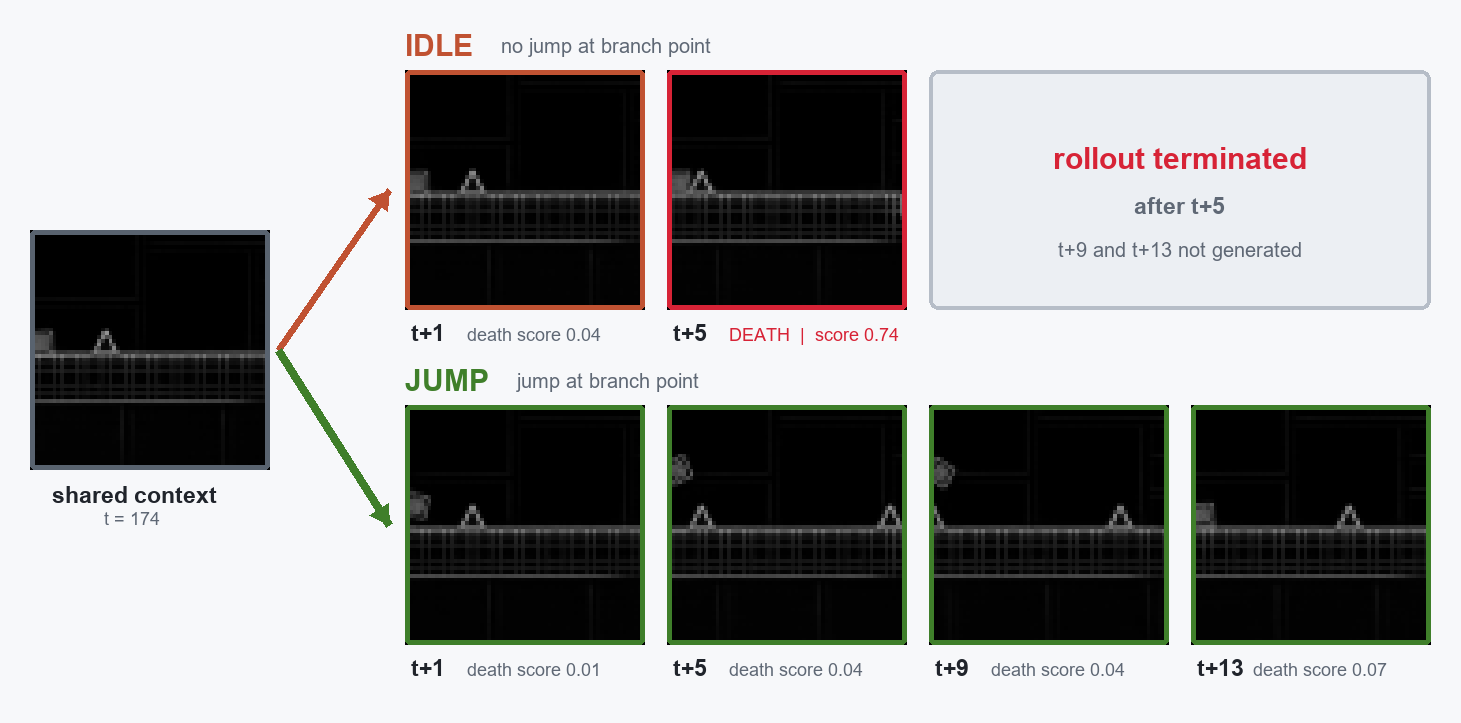
\includegraphics[width=0.82\textwidth]{figures/continuation.pdf}
  \caption{Greedy continuations from one reconstructed four-frame prefix; only the first future action differs. At \(t+1,t+5,t+9,t+13\), the jump branch clears the spike. The idle branch terminates at \(t+5\) (death score 0.74), so later frames are not generated.}
  \label{fig:continuation}
\end{figure}

\subsection{Design diagnostics}
\label{sec:ablations}

Table~\ref{tab:diagnostics} condenses engineering variants explored before freezing the system.
Because the variants span successive development stacks, the table records engineering choices rather than controlled architectural rankings.

\begin{table}[ht!]
  \centering
  \footnotesize
  \caption{Pre-freeze design diagnostics from successive development stacks. ``Live'' denotes real-game progress in local evaluation.}
  \label{tab:diagnostics}
  \begin{tabular}{p{0.20\textwidth}p{0.48\textwidth}p{0.17\textwidth}}
    \toprule
    Variant & Observed outcome & Decision \\
    \midrule
    PPO without BC (earlier stack) & Same latent plateau, about 2,000 more iterations (\(\approx6\) A100 hours); BC takes about 5 minutes. & Keep BC. \\
    Transformer width 512 & Better CE/contrastive metrics, no live gain, slower training. & Use width 384. \\
    MLP on \(\mathbf h_t\) only & PPO was 2--5\(\times\) faster with a smaller train--eval gap, but local live progress was worse. & Keep grid input. \\
    \bottomrule
  \end{tabular}
\end{table}

\FloatBarrier
\section{Limitations}
\label{sec:limitations}

DashVMC is a single-game study with binary actions and deterministic layouts.
The three controller seeds share one frozen tokenizer and world model, and the held-out evaluation covers one community layout.
IRIS and DIAMOND were not trained on the DashVMC corpus, so Table~\ref{tab:transition-latency} compares generative transition cost rather than matched Geometry-Dash control.
SLS remains a local design choice: it was selected from a single Geometry-Dash development comparison and underperformed hard CE in final return in a matched five-seed IRIS/Pong diagnostic.
The decoded continuations can drift over long horizons, and successive dataset doublings suggest that the model remains data-limited.
Finally, the latency results are specific to the tested GPU and 64-pixel edge observations.

\section{Conclusion}
\label{sec:conclusion}

DashVMC shows that a lightweight and specialized world model can support both low-latency imagined transitions and live reactive control in a timing-sensitive game.
Across three controller seeds, PPO improves mean live survival over its exact retained parent BC on all three official levels for every seed and preserves that direction on a late Level-1 copy and one custom held-out community level, while the optimized capture-to-action path sustains a 60-FPS live cadence on a consumer GPU despite 30-FPS training data.
A matched-prefix intervention shows that the model's visual future responds to the tested action change, and interactive examples show that those dynamics can produce open-ended, plausible level continuations.

\ifdashvmcsubmission\else
  \section*{Acknowledgments}
  We thank Florian Yger for valuable discussions and careful feedback on earlier versions of this manuscript.
  We thank Ma{\"e}l Planchot for contributing gameplay data.
  The NVIDIA A100 and H200 GPUs used for primary and controller-replication training were provided by MesoNet (CRIANN, Rouen) through the Representation Learning course at INSA Rouen Normandy.
  Geometry Dash is developed by RobTop Games.
\fi

\bibliographystyle{\dashvmcbibliographystyle}
\bibliography{references}

\ifdashvmcsubmission
  \newpage
  \section*{Paper Checklist}

\begin{enumerate}

\item {\bf Claims}
    \item[] Answer: \answerYes{}
    \item[] Justification: The abstract and introduction state the main claim as policy improvement learned in a frozen action-conditioned world model transferring beyond its behavioural-cloning initialization to live Geometry Dash control. They also scope the real-time deployment and held-out-layout evidence.

\item {\bf Limitations}
    \item[] Answer: \answerYes{}
    \item[] Justification: Section~\ref{sec:limitations} discusses the single-game and binary-action scope, one held-out layout within supported mechanics, one frozen tokenizer/dynamics-model seed, long-rollout fidelity, the small extended diagnostic cohort, and hardware dependence.

\item {\bf Theory assumptions and proofs}
    \item[] Answer: \answerNA{}
    \item[] Justification: The paper does not include theoretical results. SLS is an empirical method.

\item {\bf Experimental result reproducibility}
    \item[] Answer: \answerYes{}
    \item[] Justification: Section~\ref{sec:setup} provides the collection and split procedure, training details, controller hyperparameters, seeds, checkpoint-selection rules, and live protocol. Code, frozen tokenizer/world-model checkpoints, raw per-attempt results, per-seed controller hashes and provenance, an immutable reported-code snapshot, and a sequential reproduction recipe are available; the identifying repository URL is omitted from this double-blind manuscript.

\item {\bf Open access to data and code}
    \item[] Answer: \answerYes{}
    \item[] Justification: Code, the dataset, frozen base-model checkpoints, raw live results, and derived paired tables are publicly available, and the collection procedure is described in Section~\ref{sec:setup}. The identifying repository URL is withheld during double-blind review and will be restored in the camera-ready version.

\item {\bf Experimental setting/details}
    \item[] Answer: \answerYes{}
    \item[] Justification: Section~\ref{sec:setup} specifies the material model and optimization hyperparameters, schedules, three 15,000-iteration PPO budgets and selected iterations, logged stage times, controller seeds, and data augmentation.

\item {\bf Experiment statistical significance}
    \item[] Answer: \answerYes{}
    \item[] Justification: The draft reports three exact parent-BC/PPO controller pairs with 25 scored attempts per frozen policy-level on three official and two auxiliary layouts, sample standard deviations, and attempt-level PPO-minus-BC bootstrap intervals. Individual seed results and the three paired controller-seed differences are reported separately rather than pooling attempts; official-level mean, IQM, and empirical-reference gap additionally receive seed-level stratified-bootstrap intervals. This is conditional replication under one frozen tokenizer/world-model seed, not full end-to-end training uncertainty.

\item {\bf Experiments compute resources}
    \item[] Answer: \answerYes{}
    \item[] Justification: The tokenizer and world model were trained sequentially on a single NVIDIA A100 GPU; the three controller replications ran sequentially on a single H200 at a time; live deployment and latency evaluation used an RTX 2060 (PyTorch 2.11.0+cu126). Section~\ref{sec:setup} reports the relevant budgets and protocols.

\item {\bf Code of ethics}
    \item[] Answer: \answerYes{}
    \item[] Justification: The research involves no human subjects, sensitive data, or dual-use concerns.

\item {\bf Broader impacts}
    \item[] Answer: \answerNA{}
    \item[] Justification: This work applies to a single-player video game with no direct societal impact.

\item {\bf Safeguards}
    \item[] Answer: \answerNA{}
    \item[] Justification: The released model is a small world model for a video game and poses no misuse risk.

\item {\bf Licenses for existing assets}
    \item[] Answer: \answerYes{}
    \item[] Justification: All referenced works are properly cited. Geometry Dash is a commercial game by RobTop Games; gameplay data was collected from a legally purchased copy.

\item {\bf New assets}
    \item[] Answer: \answerYes{}
    \item[] Justification: Code, the collected dataset, frozen base-model checkpoints, raw evaluation artifacts, and controller-checkpoint hashes are released with documentation under the repository's open-source terms.

\item {\bf Crowdsourcing and research with human subjects}
    \item[] Answer: \answerNA{}
    \item[] Justification: No crowdsourcing or human subjects research was conducted.

\item {\bf Institutional review board (IRB) approvals or equivalent for research with human subjects}
    \item[] Answer: \answerNA{}
    \item[] Justification: No human subjects research was conducted.

\item {\bf Declaration of LLM usage}
    \item[] Answer: \answerYes{}
    \item[] Justification: OpenAI Codex was used to help restructure and edit the manuscript. The authors verified the resulting text, figures, numerical claims, and references; LLMs were not part of the methodology or experiments.

\end{enumerate}

\fi

\end{document}
